% preamble and style file for M&R lecture slides
\documentclass[11.5pt,sans,english]{beamer}

\usetheme{EastLansing}
\usecolortheme{lily}

\usepackage[most]{tcolorbox}

\usepackage{verbatim}
%\usepackage{ulem}
%\usepackage{fontawesome}
%\usepackage{tikz}
%\usepackage{pifont}
%\usepackage{tabularx}
\usepackage{array,booktabs,xcolor,colortbl,multirow,rotating,amssymb}
%\usepackage{amsmath}
% \usepackage{vwcol}
% \usepackage[T1]{fontenc}

  
\newcommand\vect[1]{\underline{\mathbf{#1}}}
\newcommand\unitvect[1]{\hat{\boldsymbol{#1}}}
%\newcommand\hatdot[1] { \hat{ \dot{ \boldsymbol{#1} } } }

\newtcbox
{\keyc}{on line,arc=2pt, colback=yellow!30!white, colframe=yellow!30!black, before upper={\rule[-3pt]{0pt}{10pt} },boxrule=1pt,boxsep=0pt,left=6pt,right=6pt,top=2pt,bottom=2pt,}

\newtcbox
{\keyb}{on line,arc=1pt, colback=blue!30!white, colframe=blue!30!black, before upper={\rule[-3pt]{0pt}{10pt} },boxrule=1pt,boxsep=0pt,left=6pt,right=6pt,top=2pt,bottom=2pt,}

\newtcbox
{\keyl}{on line,arc=1pt, colback=pink!30!white, colframe=blue!30!black, before upper={\rule[-3pt]{0pt}{10pt} },boxrule=1pt,boxsep=0pt,left=6pt,right=6pt,top=2pt,bottom=2pt,}

\newtcbox
{\keyw}{on line,arc=1pt, colback=red!30!white, colframe=blue!30!black, before upper={\rule[-3pt]{0pt}{10pt} },boxrule=1pt,boxsep=0pt,left=6pt,right=6pt,top=2pt,bottom=2pt,}

\newtcbox
{\keya}{on line,arc=1pt, colback=purple!30!white, colframe=blue!30!black, before upper={\rule[-3pt]{0pt}{10pt} },boxrule=1pt,boxsep=0pt,left=6pt,right=6pt,top=2pt,bottom=2pt,}

\newtcbox[auto counter,number within=section]
{keyf}
{
enhanced,
on line,
  boxsep=0pt,
  left=6pt,right=6pt,top=2pt,bottom=2pt,
  arc=5pt,
  boxrule=1pt,
  rightrule=38pt,
colback=green!10!white, 
colframe=green!50!black, 
title=\thetcbcounter,
detach title,
overlay unbroken and first ={
    \node[%rotate=90,
          %minimum width=1cm,
          anchor=south,
          font=\sffamily\bfseries\tiny,
          %yshift=-10pt,
          yshift=-5pt,
          xshift=-20pt,
          white]
    at (frame.east) {\thetcbcounter};
  }
}


\usepackage{xcolor}

%\usepackage{hyperref}
%\hypersetup{
%  pdfauthor={Lily Asquith},
%  urlcolor=blue,
%  colorlinks=true,
%  linkcolor=blue,
%  bookmarks=true
%}

%---------------------------------------------%
%              LILY'S COLOURS           %
%---------------------------------------------%
\definecolor{Wash}{RGB}{204,204,204}
%\definecolor{Pinky}{RGB}{254,200,254}%violet
\definecolor{Pinky}{RGB}{219,	240,	253}%violet
\definecolor{Bluey}{RGB}{0,190,255}%deep sky blue
\definecolor{DarkGrey}{RGB}{28,66,137}%dar grey
\definecolor{SussexWhite}{RGB}{253,255,254}%dar grey
\definecolor{LightGray}{RGB}{184,184,255}
\definecolor{YesGreen}{RGB}{0,128,0}
\definecolor{NoRed}{RGB}{250,0,0}



\definecolor{myred}{RGB}{255,153,153}
\definecolor{myorange}{RGB}{255,204,153}
\definecolor{myyellow}{RGB}{255,255,153}
\definecolor{mygreen}{RGB}{153,255,153}
\definecolor{mycyan}{RGB}{153,255,255}
\definecolor{myblue}{RGB}{153,204,255}
\definecolor{myviolet}{RGB}{153,153,255}
\definecolor{mypurple}{RGB}{204,153,255}
\definecolor{mypink}{RGB}{255,204,255}
\definecolor{mycoral}{RGB}{255,153,204}

%-----------------------------------------------------%
%              LILY'S COLUMN TYPES          %
%-----------------------------------------------------%
\newcolumntype{a}{>{\raggedright\arraybackslash}l}	
\newcolumntype{q}{>{\raggedright\arraybackslash}m{8cm}} 

%--------------------------------------------%
%              LILY'S SYMBOLS          %
%--------------------------------------------%
\newcommand{\dfinger}{\large{\textcolor{black}{\ding{43}}}\scriptsize}
\newcommand{\dstar}{\large{\textcolor{black}{\ding{76}}}\scriptsize}
\newcommand{\dwrite}{\large{\textcolor{black}{\ding{45}}}\scriptsize}
\newcommand{\ddiamond}{\small{\textcolor{DarkGrey}{\ding{117}}}\scriptsize}
\newcommand{\ddiamondwhite}{\small{\textcolor{SussexWhite}{\ding{117}}}\scriptsize}
\newcommand{\experiment}{\small{\textcolor{magenta}{\faCogs }}\scriptsize}
\newcommand{\watchit}{\textcolor{blue}{ \faYoutube}}


\makeatletter
\newcommand\notsotiny{\@setfontsize\notsotiny{6.5}{7.5}}
\makeatother


% 
\title[ Intro to Quantum Physics]{Intro to Quantum Physics F3241}
%\subtitle{\textbf{Part 3: Blackbody Radiation}}
\author[Dr Lily Asquith (Lily)]{ Dr Lily Asquith (Lily)}
\date[Week 3]{ Week 3}
\logo{

\includegraphics[width=1.5cm]{../../utils/uslogo.jpg}
}


\begin{document}


\begin{frame}
\titlepage
\end{frame} 

 %-----------------------------------------------------------%
 % 1 Kinematics                                                 %
 %-----------------------------------------------------------%
\section{I2Q Part 3: Blackbody Radiation}
\begin{frame}
\frametitle{Blackbody Radiation} 
\normalsize

This week's topics:\\[3ex]

\begin{itemize}
\item[3.1] Blackbody Radiation\\[3ex]
\item[3.2] The Ultraviolet Catastrophe, Planck to the rescue\\[3ex]
\end{itemize}

Your homework questions for this week are on canvas - please complete these by the end of the week.
\end{frame} 
 
 
\begin{frame}{Temperature: observations}
\small
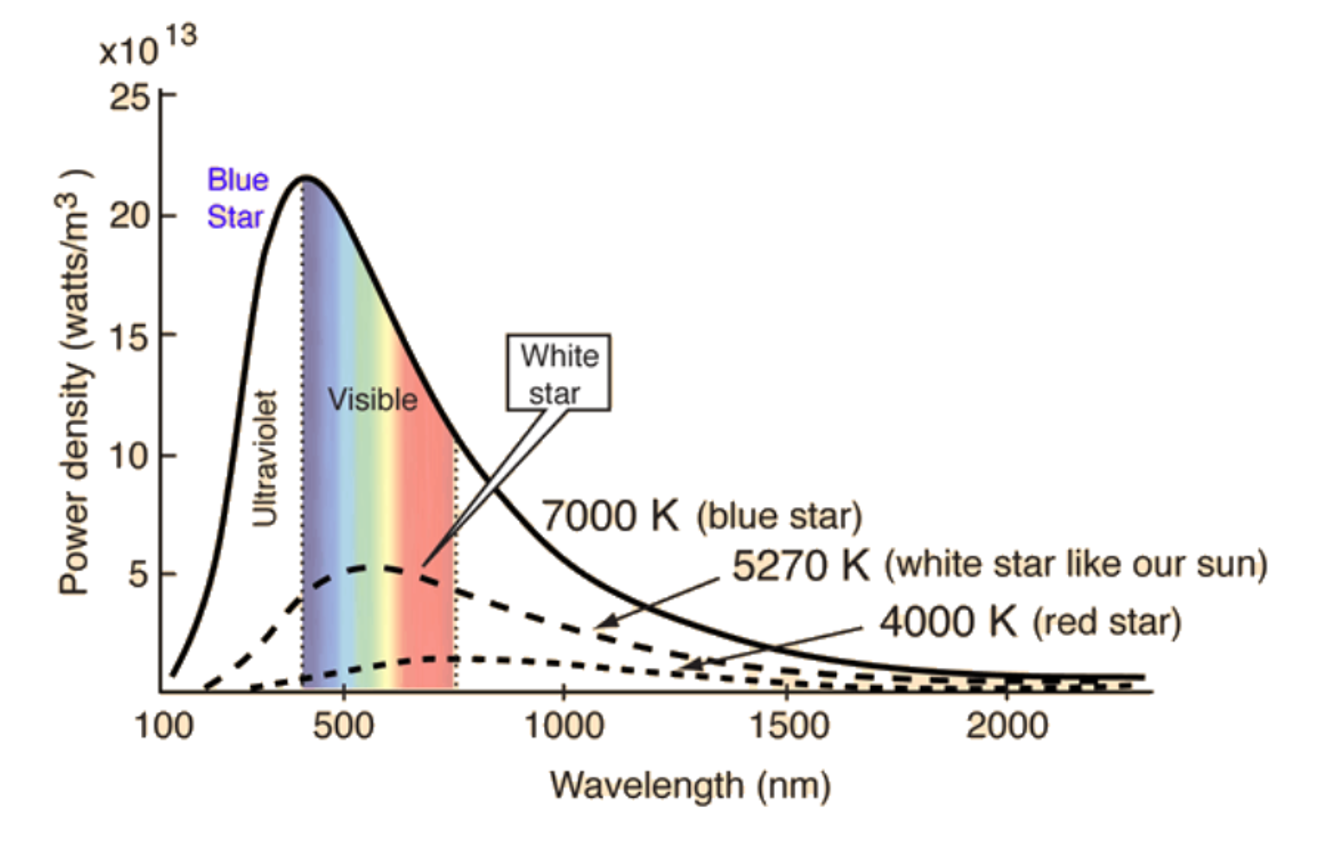
\includegraphics[scale=0.45]{bbspectrum}

Let's do a quiz: pollev.com/ilovephysics

\end{frame}


\begin{frame}{Wien's Law \& Stefan-Boltzman Law}

\small
The Peak Wavelength $\lambda_{P} \sim T^{-1}$. \\[1ex]

Wien's law: $\lambda_{P} = \sigma T^{-1}$, where $\sigma = 2.90 \times 10^{-3}$ [units?] \\[8ex]

The Peak Power Density $R_{P} \sim T^{4}$.\\[1ex]
Stefan-Boltzman Law: $R_{P} = k T^{4}$, where $k = 5.67 \times 10^8 $ Wm$^{-2}$\\[8ex]

Note that astronomers use really silly units.

\end{frame}

\begin{frame}{Silly Astronomers}
\small
From \href{https://en.wikipedia.org/wiki/Radiant_intensity}{Wikipedia: Radiant\_intensity} with a page search for "confusing":

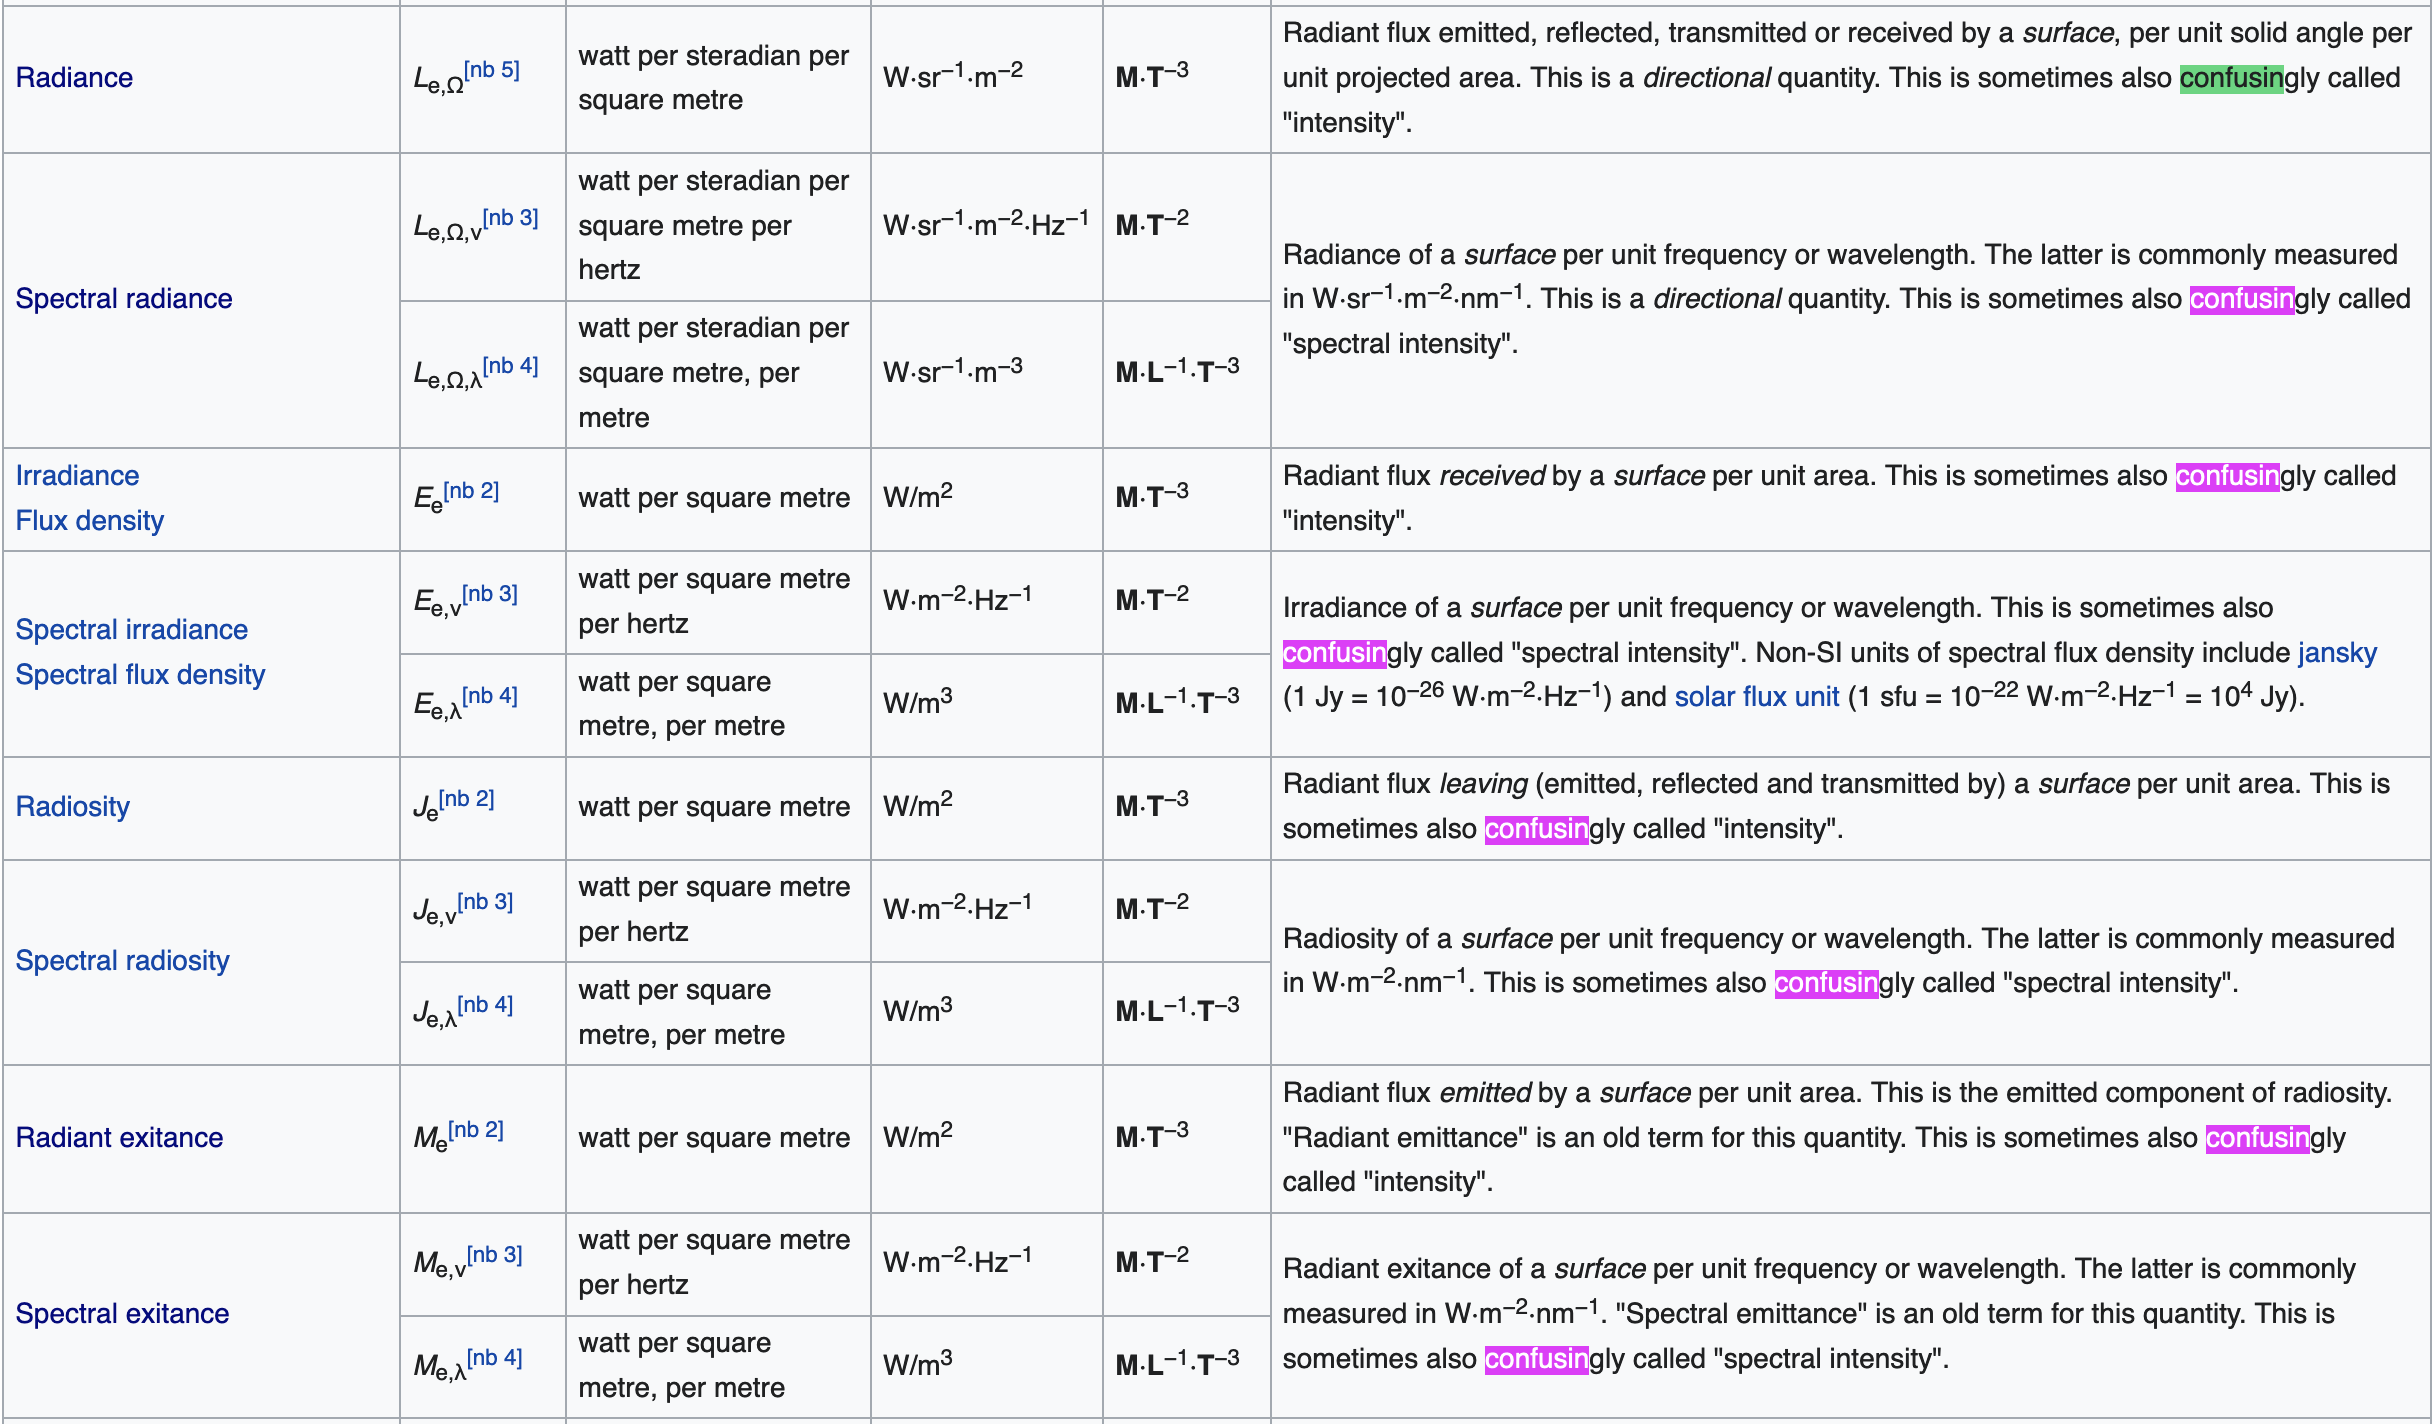
\includegraphics[scale=0.25]{astrotards}

\end{frame}

\subsection{The Ultraviolet Catastrophe, Planck to the rescue}
%
%
\begin{frame}{Energy Density: The Rayleigh-Jeans law}
\small
We can understand the blackbody spectrum in pieces, but what about the whole thing?\\[1ex]
\begin{columns}
\begin{column}{0.6\textwidth}

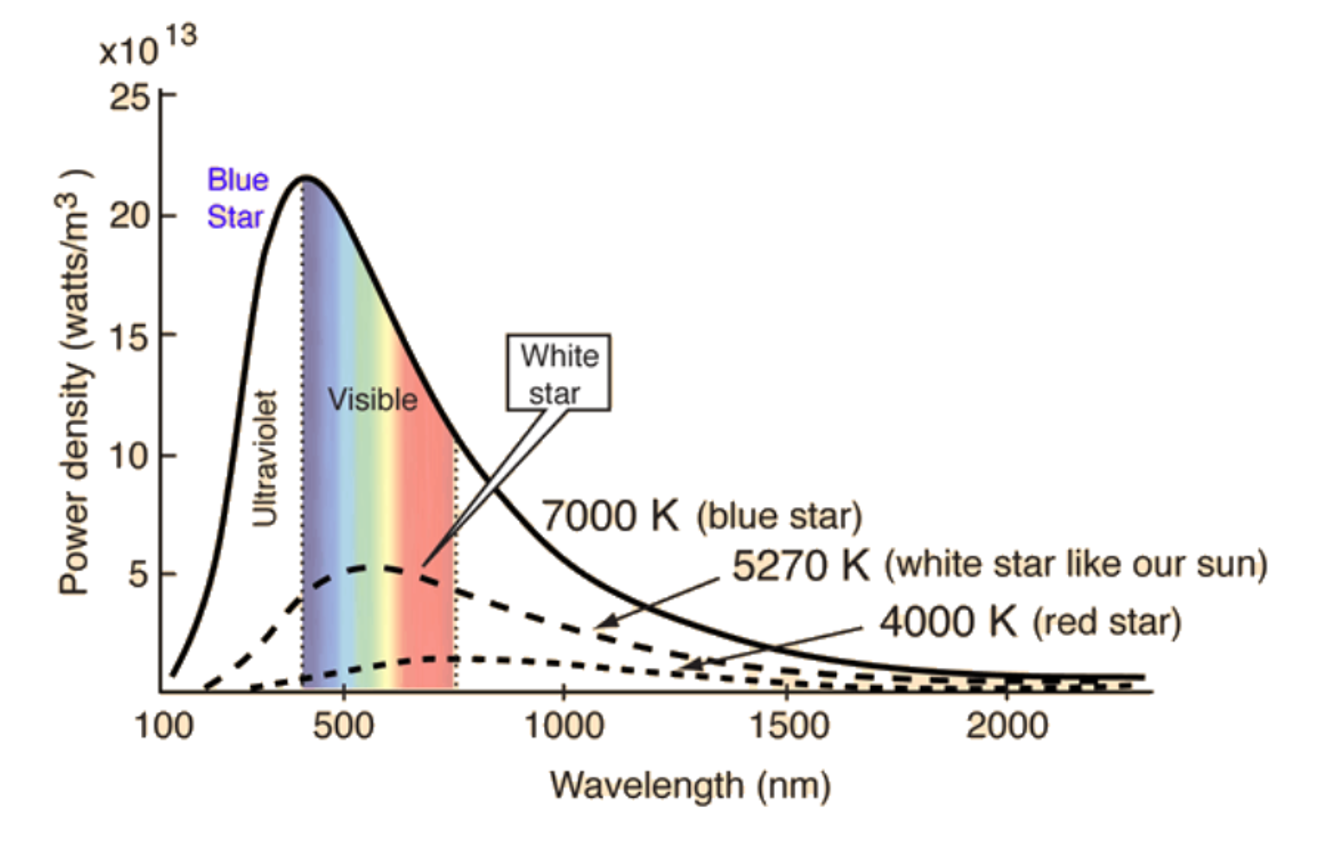
\includegraphics[scale=0.3]{bbspectrum}
\end{column}
\begin{column}{0.4\textwidth}
R-J Law: $U(T) = \frac{8\pi}{\lambda^4} k_B T$\\ [1ex]
$where$\\[1ex]
 $k_B = 1.38\times10^{-23}$ JK$^{-1}$\\[2ex]
Let's analyse this...\\[6ex]
\vspace{4cm}

\end{column}
\end{columns}
\end{frame}


\begin{frame}{The UV catastrophe: Aargh!}
\small
Classical Physics has failed us!
\begin{columns}
\begin{column}{0.6\textwidth}

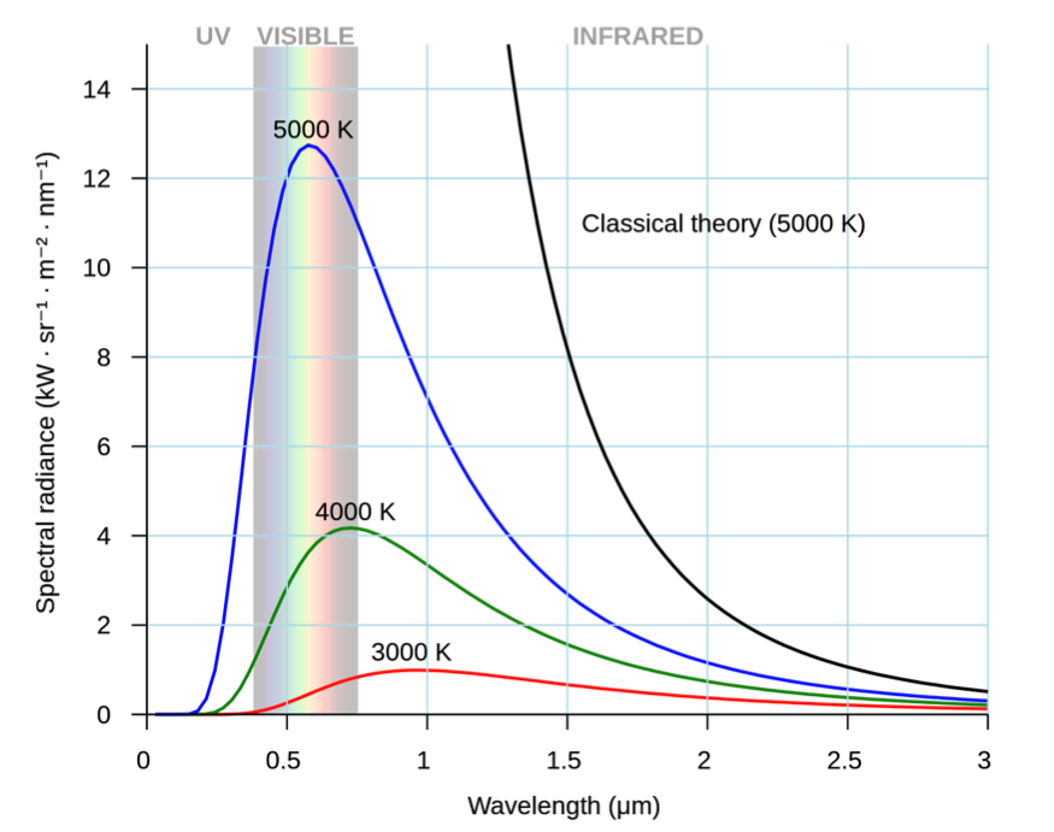
\includegraphics[scale=0.3]{uvcatas}
\end{column}
\begin{column}{0.4\textwidth}
R-J Law: $U(T) = \frac{8\pi}{\lambda^4} k_B T$\\ [1ex]
$where$\\[1ex]
 $k_B = 1.38\times10^{-23}$ JK$^{-1}$\\[2ex]
Let's analyse this...\\[6ex]
\vspace{4cm}

\end{column}
\end{columns}


\end{frame}


\begin{frame}{Relating Frequency, Wavelength, Speed}
\small

The wavelength $\lambda$\\[1ex]
The frequency $f$\\[1ex]
The speed $c$\\[1ex]

\end{frame}


\begin{frame}{Planck's ``Solution''}
\small
R-J Law: $U(T) = \frac{8\pi}{\lambda^4} k_B T$\\[2ex]
Does not agree with countless observations\\[2ex]
The theory (classical) to be modified somehow if it is to describe the data\\[2ex]
Planck found that if he insisted \textbf{the energy only take discrete values}, he got this modification for free.\\[2ex]

Allowed Energy $E = $ [some integer n] x [some constant h] x [ frequency]\\[1ex]

Planck Law: $U(T) = \frac{ 8\pi }{\lambda^4} \frac{hc}{ \lambda ( e^{(hc/\lambda)k_B T} -1)}$ \\[2ex]


This Planck formula of the `energy density' perfectly matched the observations, and solved the UV catastrophe.\\[1ex]


\end{frame}


\begin{frame}{Allowed Energies}
\small

Allowed Energy $E = $ [n] x [h] x [f] =  [n] x [h] x [ $\frac{c}{\lambda}$ ]\\[1ex]

Consider three wavelengths of em radiation:\\[1ex]

10 m (radio)\\ % 1240/10e9 = 1.24e-07, 

500 nm (visible light)\\ % 1240/500 =  2.48 

100 pm (x-ray)\\ [1ex] % 1240/0.1 = 12400

If $hc = 1240 $ eV nm, what is the smallest ($n=1$) allowed energy in eV?\\[2ex]

\textbf{Note!}\\[1ex]
Planck did not think his restriction of Energies using E=nhf was anything more than a mathematical trick.\\[1ex]
It was Einstein who realised the physical importance of this, and coined the term `Planck's constant' for h.\\[1ex]
\end{frame}


 
\end{document}